\section{Durchführung}
\label{sec:Durchfuehrung}

\subsection{Vorbereitungsaufgaben}
%\label{subsec:Vorbereitungsaufgaben} gibt in V353 keine Vorbereitungsaufgaben



\subsection{Aufgaben}
\label{subsec:Aufgaben}

In Teil \textbf{a)} soll die Zeitkonstante des RC-Gliedes mit Hilfe der Schaltung in
---noch einfügen--- bestimmt werden. 
Dazu werden Auf- und Entladevorgänge des Kondensators 
durch eine Rechteckspannung herbeigeführt und auf dem Oszilloskop die Kondensatorspannung in 
Abhängigkeit davon beobachtet.

Die Teilaufgabe \textbf{b)} sieht vor, dass man die Generatorspannung in Sinusform umstellt.
Gemessen werden soll hier die Amplitude $A(\omega)$ der Kondensatorspannung
 $U_C = A(\omega) \cdot cos(\omega t + \varphi(\omega))$ in Abhängigkeit der Frequenz
der Sinusspannung.

\textbf{c)} ist die Bestimmung der Phasenverschiebung zwischen Kondensator- und 
Generatorspannung in Abhängigkeit von der Frequenz der Sinusspannung. Die Messwerte für \textbf{b)} und \textbf{c)} konnten in einem 
Messdurchgang genommen werden, bei dem die Frequenz in kleinen Schritten erhöht wird.

In Teilaufgabe \textbf{d)} wird bewiesen, dass die vorliegende Schaltung als Integrator genutzt werden kann.
Hierzu stellt man nacheinander eine Rechteck-, Dreieck- und Sinusspannung am Generator ein und dokumentiert 
die Kondensatorspannung, die proportional zum Integral der Generatorspannung über die Zeit sein sollte.



\subsection{Aufbau}
\label{subsec:Aufbau}

\begin{figure}
    \centering
    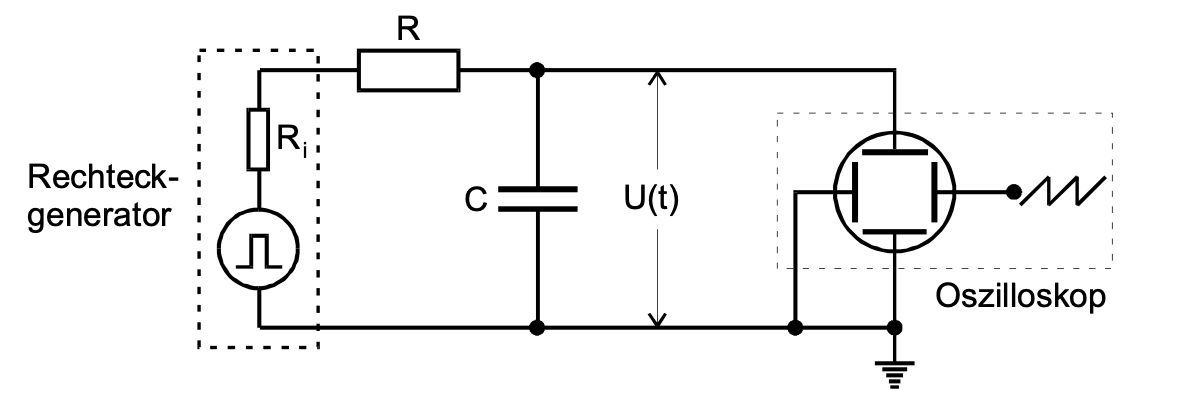
\includegraphics[height=3cm]{content/esb1.png}
    \caption{Das Ersatzschaltbild zu Teilaufgabe a)}
\end{figure}

\begin{figure}
    \centering
    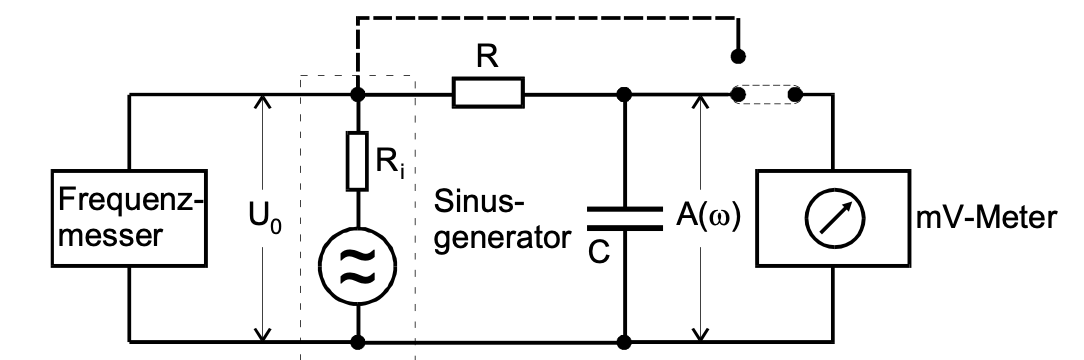
\includegraphics[height=3cm]{content/esb2.png}
    \caption{Das Ersatzschaltbild zu Aufgabe b) und c)}
\end{figure}

\begin{figure}
    \centering
    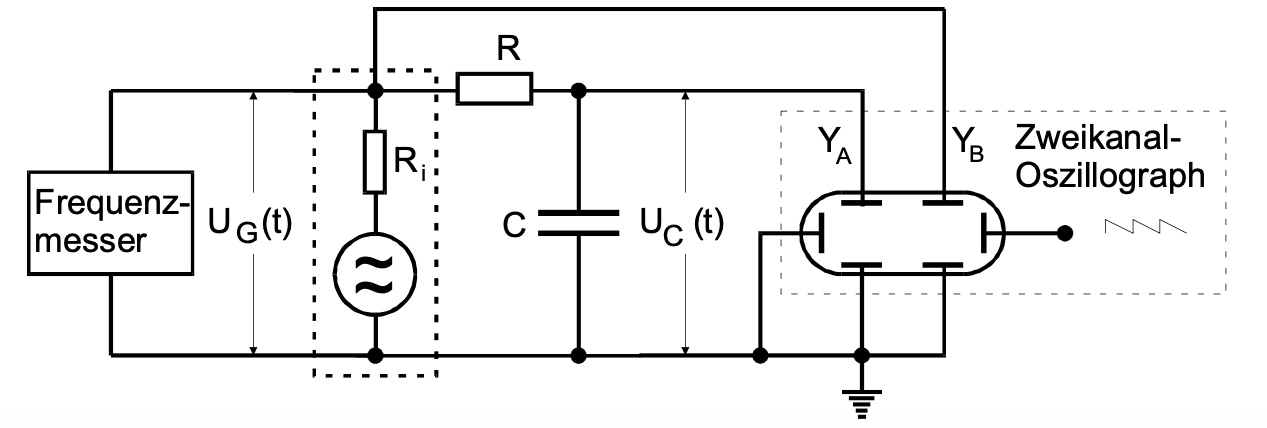
\includegraphics[height=3cm]{content/esb3.png}
    \caption{Das Ersatzschaltbild zu Teilaufgabe d)}
\end{figure}